\subsection{EulerianTrail}

\begin{definition}
    An \textbf{Eulerian trail} is a trail that passes through each edge of the graph exactly once. A graph with a closed Eulerian trail is called \textbf{Eulerian}
\end{definition}
\vspace{0.5cm}
\begin{theorem}[Euler's theorem]
    Let $G$ be a connected graph with at least 2 vertices. Then $G$ has a closed Eulerian trail iff every vertex in G has even degree
\end{theorem}
\begin{proof}
\hfill \\
    "$\implies$" \\
    Let $T$ be a closed Eulerian trail and fix an orientation on $T$. Then for every $v\in V(G)$, the incident edges can be classified as "ingoing" or "outgoing". This defines a bijection between in and outgoing edges of $T$, so $\deg(v)$ is even.\\
    "$\impliedby$" \\
    Let $T=(v_0,e_1,v_1,...,e_m,v_m)$ be a longest trail. We will prove (i) $v_0=v_m$ and (ii) $\{e_i:i\in \{1,...,m\}\}=E(G)$. (i)$+$(ii)$\iff T$ is closed Eulerian trail.\\
    \begin{enumerate}
        \item If $v_0\neq v_m$, then $v_0$ is incident to an odd number of edges in $T$. As $\deg(v_0)$ is even, there is $e\in E(G)$ incident to $v_0$ and not on $T$. We could thus append $e$ on $T$ $\lightning$ because $T$ is longest trail.
        \item Claim: $V(T)=V$. Assume otherwise there exists a vertex $v'\notin V(T)$ and $e=\{v_k,v'\}\in E(G)$ for some $k\in \{0,...,m\}$ (by connectedness). Then $(v',e,v_k,e_{k+1},v_{k+1},...,v_{m-1},e_m,v_0,e_1,...,v_{k-1},e_k)$ is a longer trail hence $V(T)=V$
        \begin{center}
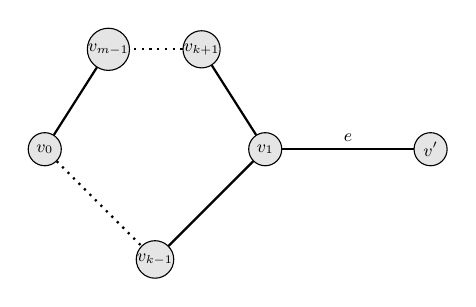
\begin{tikzpicture}[ scale=0.7,
    vertex/.style={circle, draw, fill=gray!20, minimum size=6mm, inner sep=0pt},
    every node/.style={font=\small, transform shape}
]
\def\r{2}
\node[vertex] (v1)  at ({90-335}:\r)   {$v_{m-1}$};
\node[vertex] (vm)  at ({90-25}:\r)    {$v_{k+1}$};
\node[vertex] (v2) at ({90-270}:\r)    {$v_0$};
\node[vertex] (vk)  at ({0}:\r)        {$v_1$};
\node[vertex] (vp) at (5, 0) {$v'$};
\node[vertex] (vk1) at ({-90}:\r) {$v_{k-1}$};

\draw[thick] (vk) -- node[midway, above] {$e$} (vp);
\draw[thick] (vk)--(vm);
\draw[thick] (v1)--(v2);
\draw[thick] (vk)--(vk1);
\draw[thick, dotted] (v2)--(vk1);
\draw[thick, dotted] (vm)--(v1);
\end{tikzpicture}
\end{center}
\par
        Claim: $E(T)=E$. Assume otherwise. Consider $e\in E\setminus E(1)$ and write $e=\{v_k,v_l\}$. Then $(v_k,e_{k+1},v_{k+1},...,v_{m-1},e_m,v_0,e_1,v_1,...,e_k,v_k,e,v_l)$ is a longer trail $\lightning$ 
    \end{enumerate}
\end{proof}
\vspace{0.5cm}

\begin{theorem}
    Let $G$ be a connected graph with at least two vertices. Then $G$ has an Eulerian trail iff there are precisely $0$ or two vetices of odd degree
\end{theorem}
\begin{proof}
    \hfill\\
    By the Euler's Theorem, we know that if there are $0$ vertices of odd degree then there exists an Eulerian trail (in fact a closed Eulerian trail), and if there exists a closed Eulerian trail, then all vertices have even degree.\par
    Suppose now that $G$ has exactly two vertices $x$ and $y$ of odd degree. We consider the following graph $G'$: Set $V(G')=V(G)\cup \{z\}$, where $z\notin V(G)$. Furthermore set $E(G')=E(G)\cup\{\{x,z\},\{y,z\}\}$. Clearly, every vertex has even degree in $G'$, so there exists a closed Eulerian trail. Since $z$ is only adjacent to $x$ and $y$, these are the neighbours of $z$ on the trail. Deleting the edges $\{x,z\}$ and $\{y,x\}$ from the trail yields an Eulerian trail from $x$ to $y$ in $G$. Conversely, if there is a non-closed Eulerian trail with endpoints $x$ and $y$ in $G$, then $x$ and $y$ are non-adjacent. Adding the edge $\{x,y\}$ creates a graph with a closed Eulerian trail, so all vertices have even degree by Euler's theorem. Thus $x$ and $y$ are the only verices in $G$ with odd degree.
\end{proof}